 % !TEX program = lualatex
 % https://github.com/andiac/gemini-cam
% a fork of https://github.com/anishathalye/gemini


%%%% ADJUST DIMS BEFORE PRINT
%%%% ADJUST DIMS BEFORE PRINT
%%%% ADJUST DIMS BEFORE PRINT
%%%% ADJUST DIMS BEFORE PRINT
%%%% ADJUST DIMS BEFORE PRINT
%%%% ADJUST DIMS BEFORE PRINT


\documentclass[final]{beamer}

% ====================
% Packages
% ====================

\usepackage[T1]{fontenc}
\usepackage{lmodern}
\usepackage[size=custom,width=40,height=32,scale=0.4]{beamerposter}
\usetheme{gemini}
\usecolortheme{gemini}
\usepackage{graphicx}
\usepackage{booktabs}
\usepackage{tikz}
\usepackage{pgfplots}
\pgfplotsset{compat=1.14}
\usepackage{anyfontsize}
\usepackage{caption}

% ====================
% Lengths
% ====================

% If you have N columns, choose \sepwidth and \colwidth such that
% (N+1)*\sepwidth + N*\colwidth = \paperwidth
\newlength{\sepwidth}
\newlength{\colwidth}
\setlength{\sepwidth}{0.025\paperwidth}
\setlength{\colwidth}{0.3\paperwidth}

\newcommand{\separatorcolumn}{\begin{column}{\sepwidth}\end{column}}

% ====================
% Title
% ====================

\title{SkillSync: Explainable, Efficient, and Transparent Resume Evaluation} 

\author{Maximilian Schulten \inst{1} \and Jack Alberto \inst{1} \and Tommaso Beretta \inst{1} \and William Hugus \inst{1} \and Nathaniel Hahn \inst{1} \and Dr. Shaui Xu\inst{1}}

\institute[shortinst]{\inst{1} Case Western Reserve University School of Engineering, Department of Computer and Data Sciences} %\samelineand \inst{2} Another Institute}

% ====================
% Footer (optional)
% ====================

\footercontent{
  SkillSync \hfill
  Intersections 2026, Cleveland OH \hfill
\href{mailto:null@case.edu}{\{jia15, txb341, wmh42, mls384, nrh51, sxx214\}@case.edu}}
% (can be left out to remove footer)

% ====================
% Logo (optional)
% ====================
% Refer to https://github.com/k4rtik/uchicago-poster
% logo: https://communications.admin.ox.ac.uk/communications-resources/visual-identity/identity-guidelines/the-oxford-logo

% replace with clear background -- and higher quality image
\logoright{
\includegraphics[height=0.8cm]{assets/black_cw.png}}
% \logoleft{\includegraphics[height=7cm]{logos/ox-logo.png}}

% ====================
% Body
% ====================

\begin{document}



\begin{frame}[t]
\begin{columns}[t]
\separatorcolumn

\begin{column}{\colwidth}

  \begin{block}{Abstract}

    Job searching is often a time consuming and inefficient process that relies heavily on user judgement to assess their own fit for each job opening. 
    With the rise of online job boards that everyone can access, the online job market has become overly competitive in recent years. 
    This project, SkillSync, develops a lightweight, privacy focused, and data driven system for matching resumes to job descriptions. 

    The goal of this project is to automate and improve the user experience of job searching by generating a list of job openings for which the user is most qualified for. 
    The system operates through a pipeline that includes skill extraction from the resume, job data aggregation, matching process, and generating the list of top matches. 
  \end{block}

  \begin{block}{System Outline}
    
      We divide \textbf{SkillSync} into four main steps:

    \begin{enumerate}
      \item \textbf{Skill Extraction:} The user uploads a resume and the skills are extracted while personal identifiable information is removed.
      \item \textbf{Job Aggregation:} We query multiple APIs to maximize job opportunities; each job has key features extracted.
      \item \textbf{Skill Matching:} The skills extracted during step on are matched with the job features extracted in step two. Keyword search and a matching model are applied. 
      \item \textbf{Match Presentation:} We present the ordered top matches to the user in a clean and functional UI.
    \end{enumerate}

  \end{block}

  \begin{alertblock}{Skill Extraction and Preprocesssing}

    The skill extraction modules contain the data cleaning, resume classifier and skill extraction, the result of this module is a full understanding of the users resume without and personally identifying information (PII).

    \begin{itemize}
      \item \textbf{Data Cleaning:}
          \begin{itemize}
              \item strips non-alphanumeric characters and white space
              \item uses regex and named entity recognition to obsfucate PII
              \item Removing PII eliminates implicit bias in later trained networks
            \end{itemize}

      \item \textbf{Resume Classification:}  

          \begin{itemize}
              \item Linear support vector matchine classifies resumes into 12 industry buckets
              \item Embedding transformer to vectorize the resume
              \item Achieves \textbf{>90\%} top-2 accuracy 
            \end{itemize}
      \item \textbf{Skill Extraction:} 
          \begin{itemize}
              \item spaCy PhraseMatcher used for rapid dictionary matching agaisnt 99k relevant terms
                \item GLiNER (bidirectional transformer) used to extract semantic information like education and experience
          \end{itemize}
  \end{itemize}
    

  \end{alertblock}

  \begin{block}{References and Relevant Classes}

      CSDS 132, CSDS 133, CSDS 221, CSDS 233, CSDS 293, CSDS 310, CSDS 338, CSDS 240, CSDS 356, CSDS 391

    \nocite{*}
    \footnotesize{\bibliographystyle{plain}\bibliography{poster}}

  \end{block}


\end{column}

\separatorcolumn

\begin{column}{\colwidth}

  \begin{block}{System Architecture}

    SkillSync is built as a three-tier web application. The front end is a single-page interface where users paste their resume and receive a ranked list of job matches. It communicates
  with a Flask back end that exposes two REST endpoints, /find-jobs for full pipeline execution and /score-job for scoring a single listing. The back end orchestrates a multi-stage NLP
  pipeline: resume parsing and classification, job aggregation, skill extraction, and composite scoring. All components are containerized via Docker with memory limits set to the
  resource demands of the embedded transformer models.
   % \begin{figure}
   % \centering
   %     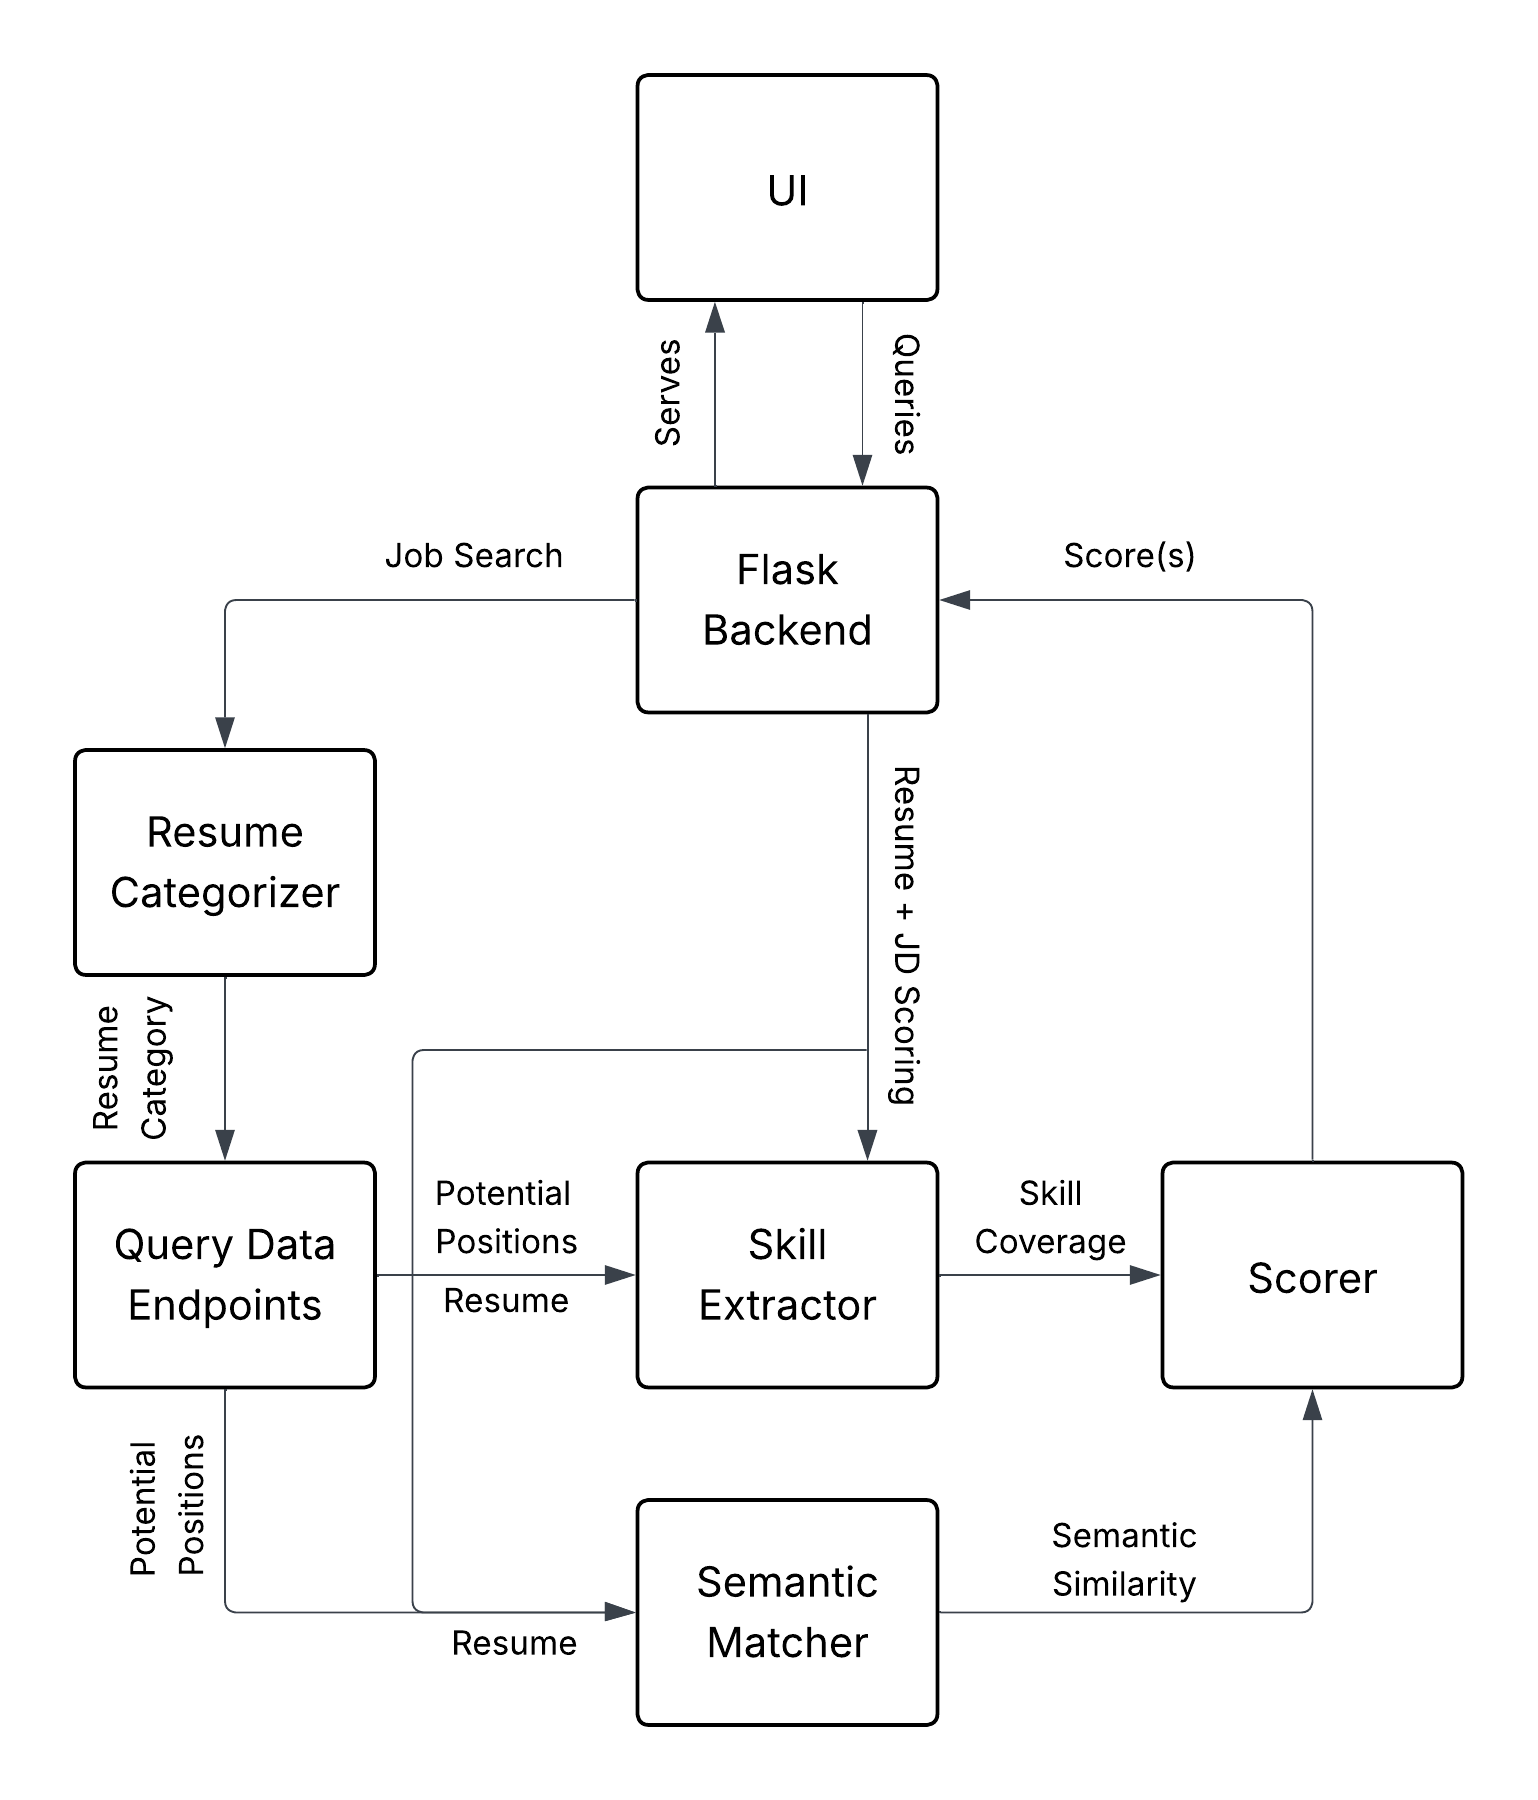
\includegraphics[width=15cm]{assets/sys_arch.png}
   %     \caption{System Architecture}

   % \end{figure}

    \begin{figure}

    \begin{columns}[c] % [c] centers the columns vertically

        % Left Pane: Single Image
        \begin{column}{0.48\textwidth}
            \centering
            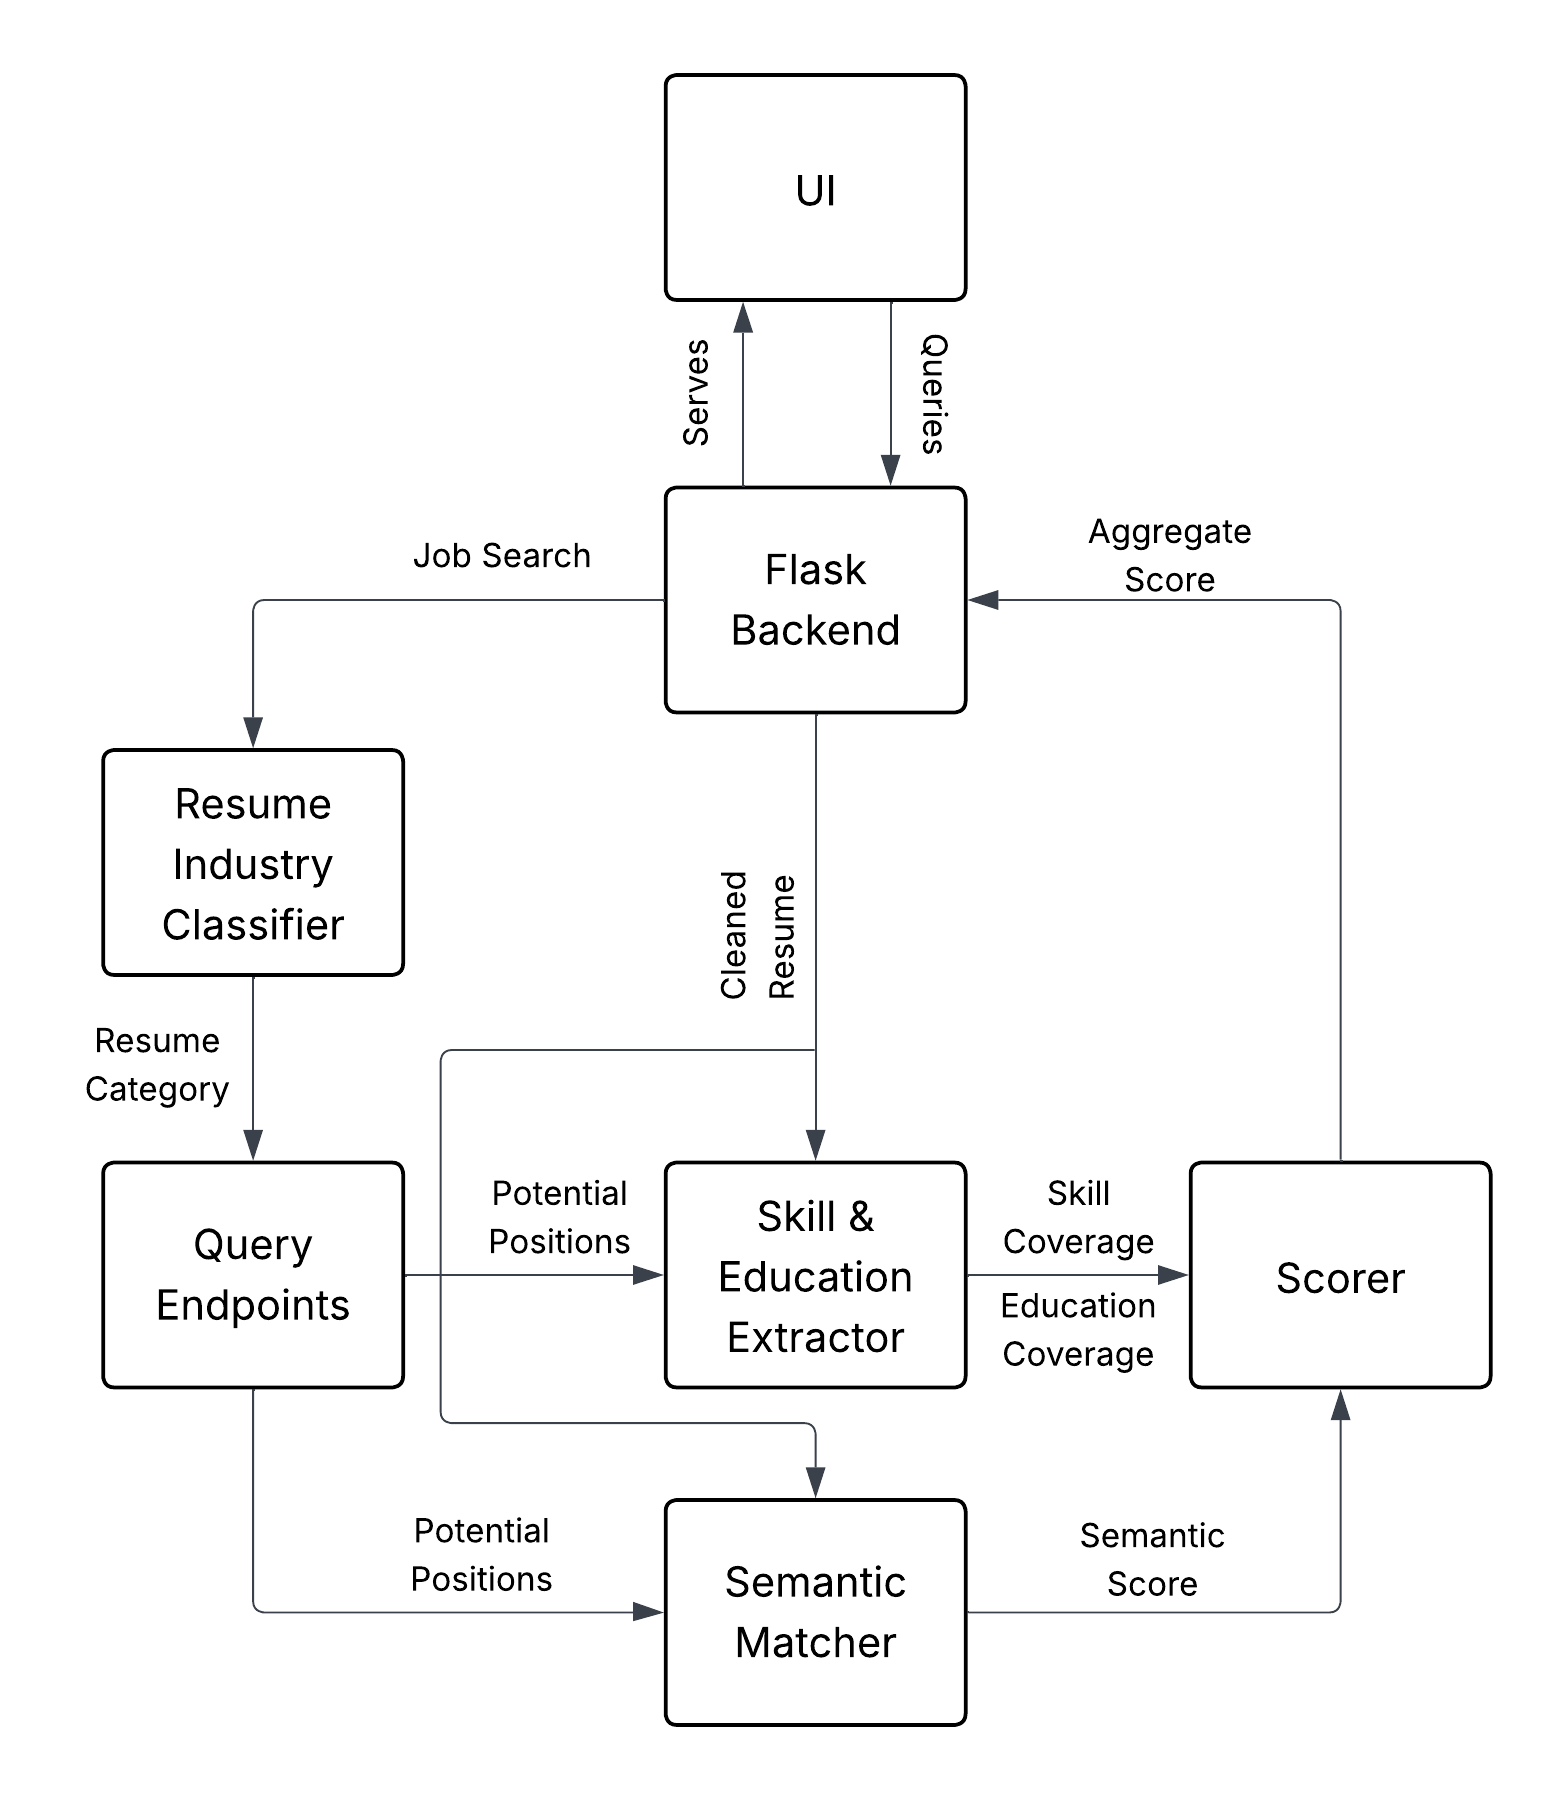
\includegraphics[width=\textwidth]{../project-assets/architecture.png}
            \captionof{figure}{System Architecture}

        \end{column}

        % Right Pane: 2x2 Grid
        \begin{column}{0.54\textwidth}
            \centering
            % Row 1
            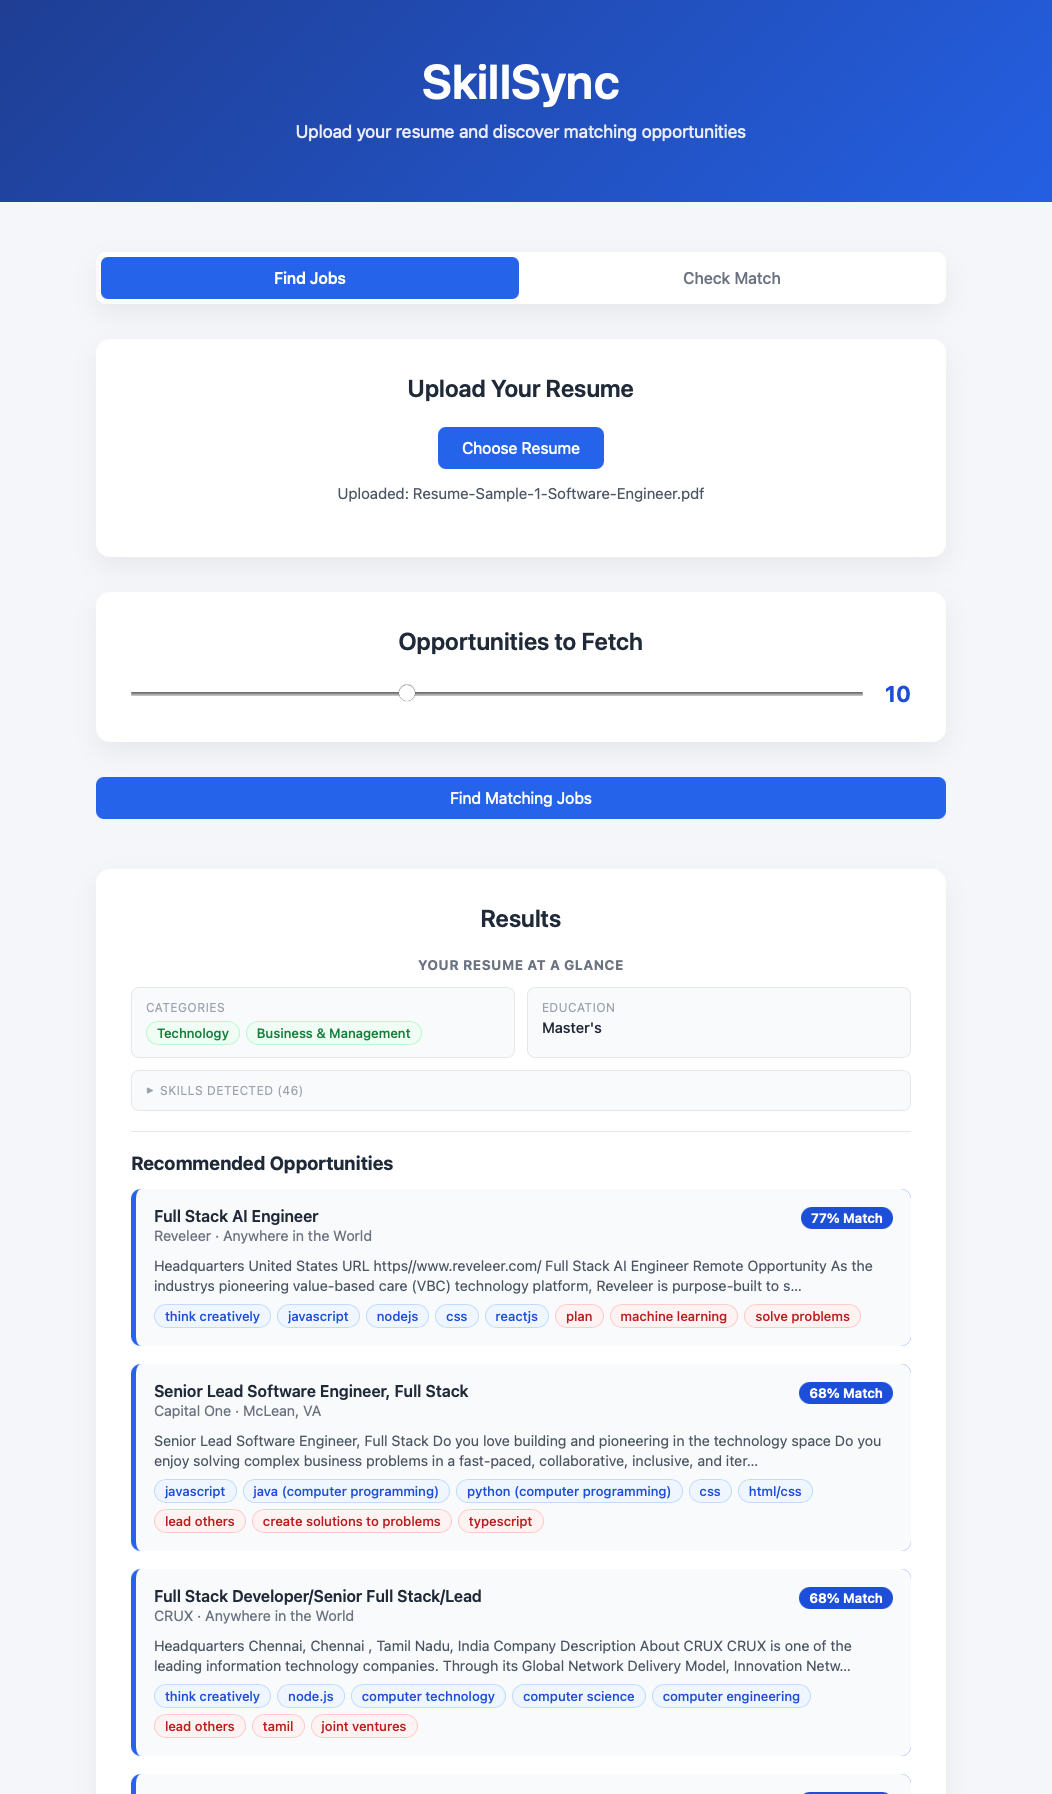
\includegraphics[width=0.45\textwidth]{assets/sized_ex1.png}
            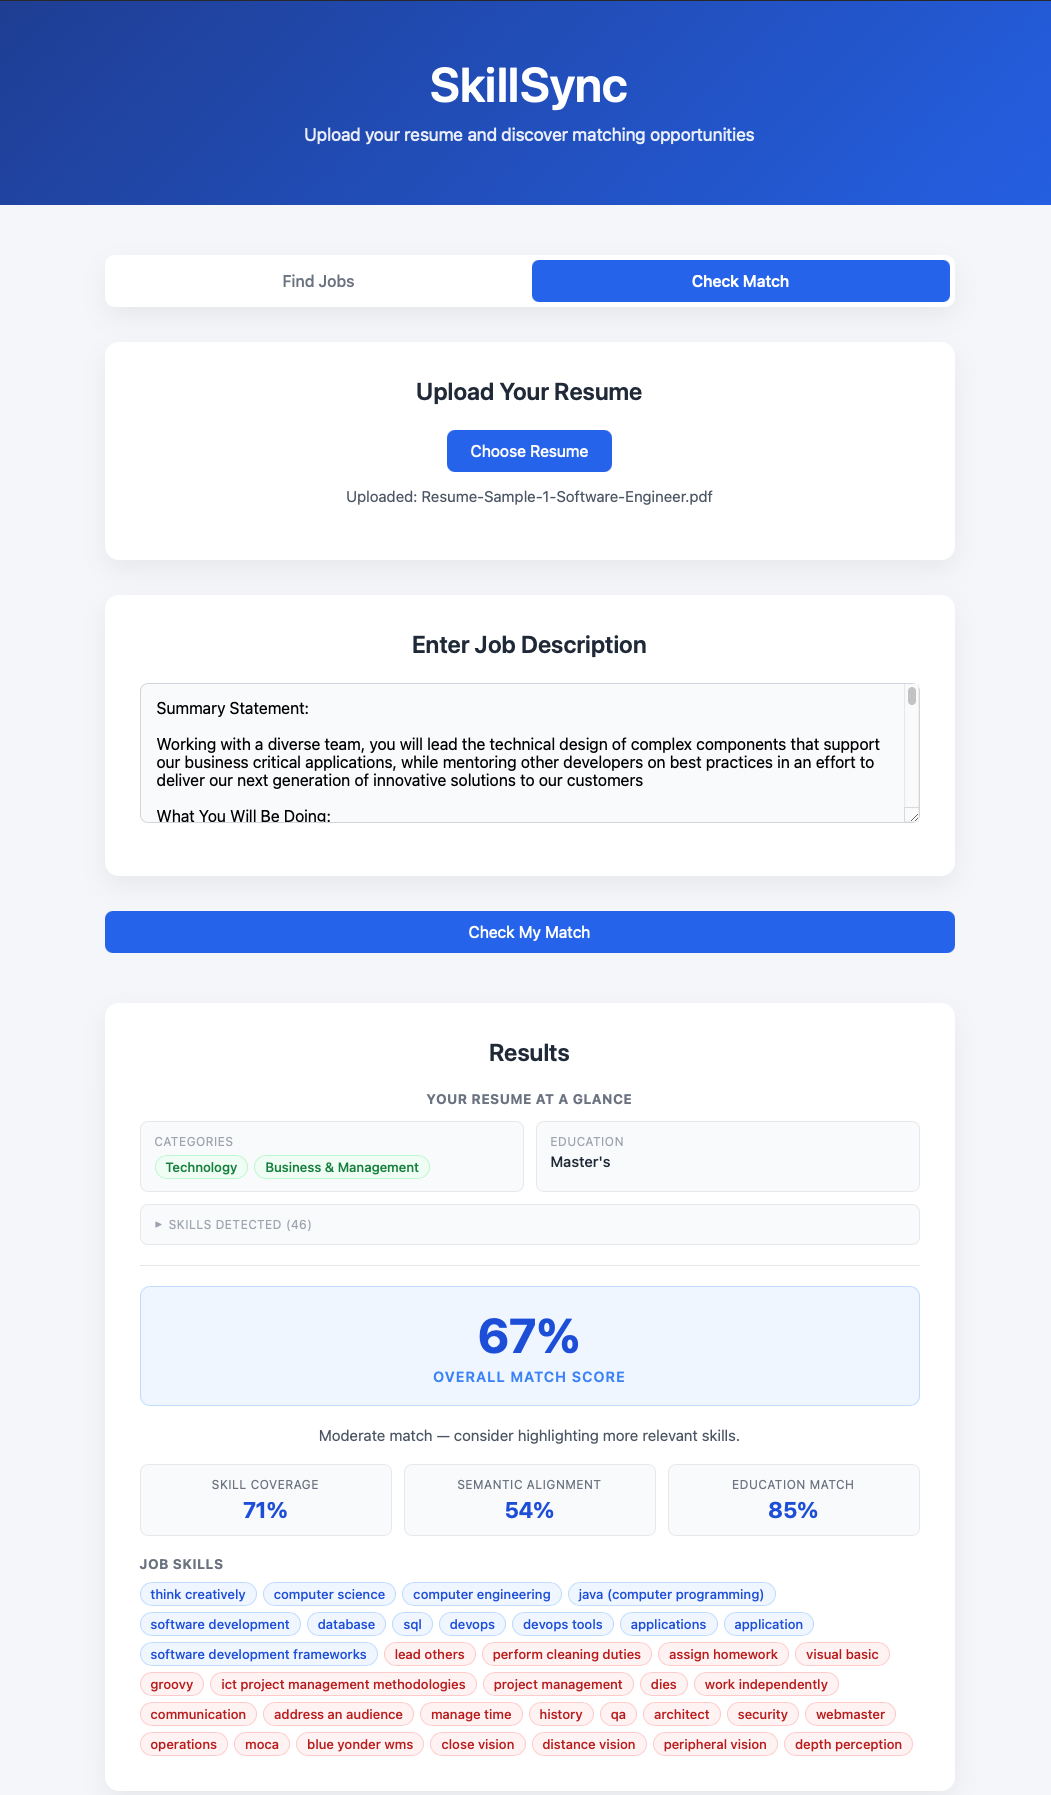
\includegraphics[width=0.45\textwidth]{assets/sized_ex2.png}

            \captionof{figure}{Front End Examples}
        \end{column}

    \end{columns}
\end{figure}


  %%% add diagram here


  \end{block}

  \begin{block}{Data Aggregation}

\begin{figure}

    \begin{columns}[c] % [c] centers the columns vertically
        
        % Left Pane: Single Image
        \begin{column}{0.48\textwidth}
            \begin{itemize}
                \item Asynchronous fetching from 8 seperate job boards, covering multiple sectors and industries 
                \item Data is normalized into a Job Object from its original schema
                \item Jobs are filtered and duplicates removed to ensure unique listings
                \item Skill extraction applied to jobs 
            \end{itemize}

        \end{column}

        % Right Pane: 2x2 Grid
        \begin{column}{0.48\textwidth}
            \centering
            % Row 1
            \centering
            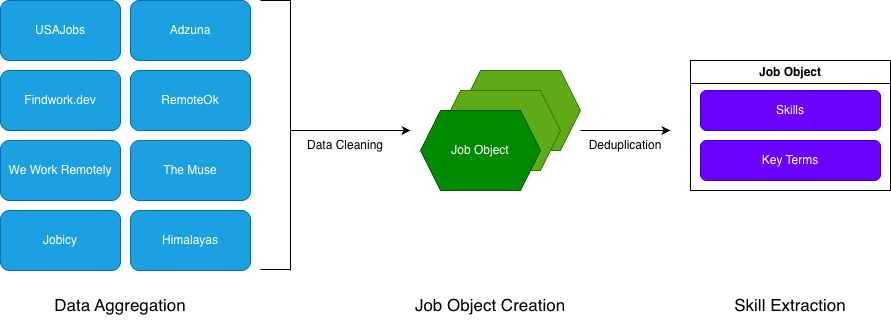
\includegraphics[width=6cm]{assets/data_agg.drawio.png}
            \caption{Data Aggregation Pipeline}            
        \end{column}
        
    \end{columns}
\end{figure}

  \end{block}

  %% add diagram 

  \begin{block}{Front End}

    The interface is minimal and clean, featuring a resume text input and a results panel. After submission, users see each job ranked by composite match score, with per-job breakdowns of
  matched skills, unmatched skill gaps, and sub-scores for skill coverage, semantic similarity, and education alignment. This transparency lets users understand why a job ranked highly
  rather than treating the score as a black box.

  \end{block}

\end{column}

\separatorcolumn

\begin{column}{\colwidth}

  \begin{exampleblock}{Matching Model}
    \small % Slightly smaller text to fit all the math on one slide
    SkillSync scores each job listing against a parsed resume using a convex
    combination of three complementary signals:

    \begin{equation}
        S_{\text{total}} = \alpha \cdot S_{\text{skill}} + \beta \cdot S_{\text{sem}} + \gamma \cdot S_{\text{edu}}, \quad \alpha + \beta + \gamma = 1
    \end{equation}

    Default weights: $\alpha = \beta = 0.45$, $\gamma = 0.1$.

    \begin{itemize}
        \item \textbf{Skill Coverage ($S_{\text{skill}}$)} \\
        Matches deterministically from databases aggregated from O*NET and ESCOU alongside a fuzzy matching system leveraging {\tt all-MiniLM-L6-v2} embeddings and cosine similarity:
        \begin{equation}
            S_{\text{skill}} = \tilde{\sigma}\left(\frac{1}{|J|} \sum_{j \in J} w\!\left(\max_{r \in R}\, \cos(e_j,\, e_r)\right)\right)
        \end{equation}
        where $w(x)$ rewards matches above threshold $\tau = 0.6$, and $\tilde{\sigma}$ applies a shifted sigmoid function to ensure saturation at acceptable raw coverage values.

        \item \textbf{Semantic Similarity ($S_{\text{sem}}$)} \\
        To capture contextual alignment beyond discrete skills, the resume and
        job description are each segmented into overlapping windows of 30 tokens
        with stride 10. The mean of per-window maximum cosine similarities
        $\bar{s}$ is mapped to a calibrated score via a normal CDF
        fit empirically to 25k+ job--resume pairs ($\mu = 0.345,\; \sigma = 0.067$):

        \begin{equation}
            S_{\text{sem}} = \Phi_{\mu,\sigma}(\bar{s}), \quad \bar{s} = \frac{1}{|W_J|}\sum_{w \in W_J} \max_{v \in W_R} \cos(e_w, e_v)
        \end{equation}

        \item \textbf{Education Coverage ($S_{\text{edu}}$)} \\
        Combines degree-level alignment and major similarity:
        \begin{equation}
            S_{\text{edu}} = 0.7 \cdot S_{\text{deg}} + 0.3 \cdot S_{\text{maj}}
        \end{equation}
    \end{itemize}

    $S_{\text{deg}}$ is a hierarchical score (1.0 if the candidate meets or
  exceeds the required degree level, 0.5 if one level below, 0.0 otherwise).
  $S_{\text{maj}}$ is the cosine similarity between embedded major strings,
  thresholded at $\tau_{\text{edu}} = 0.6$

  \end{exampleblock}


  \begin{block}{Testing and Results}
    Our project features a full pytest suite meant to ensure consistent development among a multi-person team and deployment verification. 
    These tests provide coverage across our entire build, preprocess, extract and inference modules allowing us to verify changes and catch bugs.

    An example of our results are seen the in the front end demo, along with the figure below, which describes the approximate distribution of our pipeline on a random set of $25{,}800$ resume-job combinations.
    
    \begin{figure}
    \begin{columns}[c]
        \begin{column}{0.4\textwidth}
            \centering
            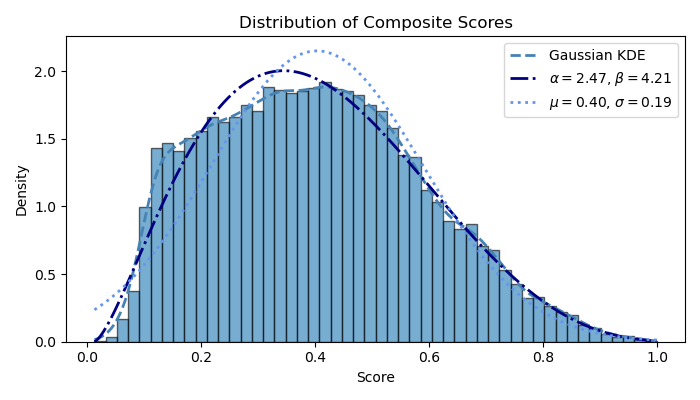
\includegraphics[width=\textwidth]{../experiments/figures/scores_dist.png}
            \captionof{figure}{Score Distribution}
        \end{column}
        \begin{column}{0.58\textwidth}
            \centering
            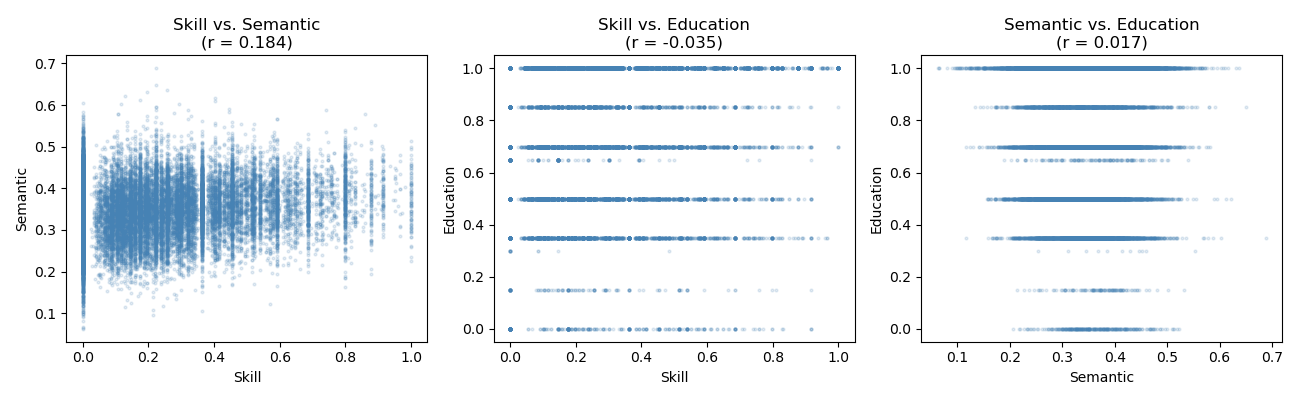
\includegraphics[width=\textwidth]{../experiments/figures/correlates.png}
            \captionof{figure}{Scoring Correlates}
        \end{column}
    \end{columns}
    \end{figure}



  \end{block}
 \begin{block}{Project Challenges}
    \end{block}



  

\end{column}

\separatorcolumn
\end{columns}
\end{frame}

\end{document}
